\documentclass{scrartcl}

\usepackage{hyperref}
\usepackage{amssymb}
\usepackage{mathtools}
\usepackage{float}
\usepackage[a4paper, left=1cm, right=1cm, top=2cm, bottom=3cm]{geometry}

\newcommand{\ffrac}[2]{\ensuremath{\frac{\displaystyle #1}{\displaystyle #2}}}

\begin{document}

\tableofcontents
\newpage

\section{Introduction: What is Artificial Intelligence}
\begin{itemize}
    \item
        What is AI? Four possible answers:
        \begin{itemize}
            \item
                Systems that think like humans
            \item
                Systems that think rationally
            \item
                Systems that act like humans
            \item
                Systems that act rationally
        \end{itemize}
    \item
        Rational behavior: doing the right thing (right thing: that which is expected to maximizing goal achiebement, given the available information)
\end{itemize}
\textbf{Rational Agents}
\begin{itemize}
    \item
        An agent is an entity that perceives and acts 
\end{itemize}
\section{Intelligent Agents: a Unifying Framework for AI}
\subsection{Agents and Environments as a Framework for AI}
\begin{itemize}
    \item
        An agent is anything that
        \begin{itemize}
            \item
                perceives its environment via sensors (means of sensing the environment)
            \item
                acts on it with actuators (means of changing the environment)
        \end{itemize}
    \item
        A \textbf{percept} is the perceptual input of an agent at a specific instant
    \item
        Any employment of the actuators of an agent is called an \textbf{action}
    \item
        The \textbf{agent function} maps from percept histories to actions $f_a: \mathcal{P}^* \rightarrow \mathcal{A}$ 
    \item
        Agent schema:
        \begin{figure}[H]
            \centering
            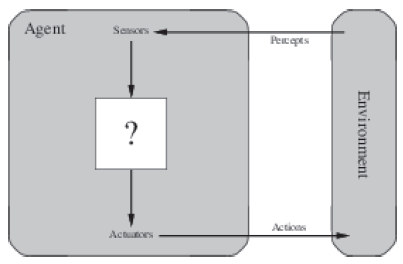
\includegraphics[scale=0.8]{figures/38}
        \end{figure}
        Different agents differ on the contents of the white box in the center
    \item
        First Idea: \textbf{Table-Driven Agents}
        \begin{itemize}
            \item
                Implement the agent funtion as a table and look up actions
            \item
                Problem: Table much to large. Even with $n$ binary percepts, we have $2^n$ actions
        \end{itemize}
\end{itemize}
\subsection{Good Behavior, Rationality}
\begin{itemize}
    \item
        Idea: Try to design agents that are successful
    \item
        A \textbf{performance measure} is a function that evaluates a sequence of environments
    \item
        An agent is called \textbf{rational}, if he chooses whichever actions maximizes the \textbf{expected value} of the performance measure given the percept sequence to date
    \item
        Rational not equal perfect
    \item
        An agent is called \textbf{autonomous}, if it doesn't rely on the prior knowledge of the designer 
    \item
        \textbf{PEAS} description of an agent:
        \begin{itemize}
            \item
                Performance measure
            \item
                Environment
            \item
                Actuators
            \item
                Sensors
        \end{itemize}
\end{itemize}
\subsection{Classifying Environments and Agents}
\begin{itemize}
    \item
        The environment type largely determines the agent design
    \item
        Dimensions by which to classify an environment ($a$: agent, $e$: environment)\\
        \begin{itemize}
            \item
                \textbf{fully observable} vs. \textbf{partially observable}: $a$'s sensors give access to the complete state of the environment
            \item
                \textbf{deterministic} vs. \textbf{stochastic}: next state of $e$ is completely determined by the current state and $a$'s actions
            \item
                \textbf{episodic} vs. \textbf{sequential}: $a$'s experience is divided into atomic episodes, where it perceives and then perfomes a single action. The next episode doesn't depend on previous ones
            \item
                \textbf{dynamic} vs. \textbf{static}: the environment can change with out an action performed by $a$
            \item
                \textbf{discrete} vs. \textbf{continuos}: the set of $e$'s states and $a$'s actions are contable
            \item
                \textbf{single-agent}: only $a$ acts on $e$
        \end{itemize}
    \item
        Real world: partially observable, stochastic, sequential, dynamic, continuous, multi-agent (worst case for AI)
\end{itemize}
\textbf{Agent types}
\begin{itemize}
    \item
        \textbf{Simple reflex agent}
        \begin{figure}[H]
            \centering
            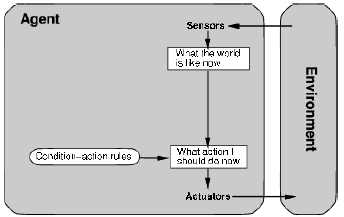
\includegraphics[scale=1]{figures/47}
        \end{figure}
        \begin{itemize}
            \item
                A simple reflex agent is an agent $a$ that only bases its actions on the last percept: $f_a: \mathcal{P} \rightarrow \mathcal{A}$
        \end{itemize}
    \item
        \textbf{Reflex agent with state}
        \begin{figure}[H]
            \centering
            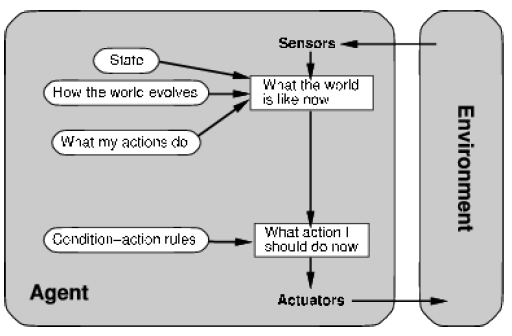
\includegraphics[scale=1]{figures/48}
        \end{figure}
        \begin{itemize}
            \item
                A stateful reflex agent (or model-based agent) whose agent funtion depends on a model of the world
        \end{itemize}
    \item
        \textbf{Utility-based agents}
        \begin{figure}[H]
            \centering
            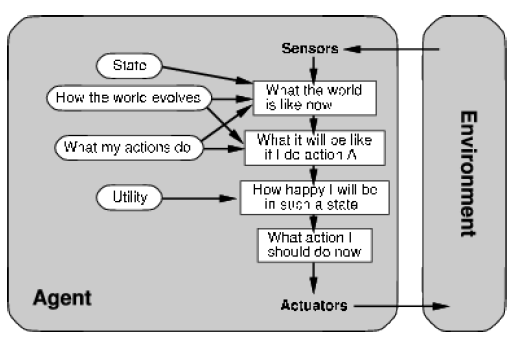
\includegraphics[scale=1]{figures/49}
        \end{figure}
        \begin{itemize}
            \item
                A utility-based agent sees a world model along with a utility function that measures its preferences among the states of that world. I chooses the action that leads to the best expected utility (averaging over all possible outcome states and weighting by the probability of the outcome)
        \end{itemize}
    \item
        \textbf{Learning agents}
        \begin{figure}[H]
            \centering
            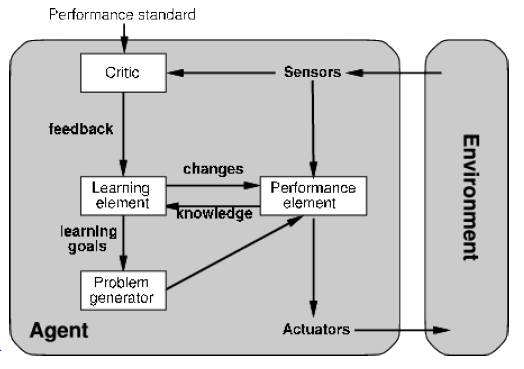
\includegraphics[scale=1]{figures/50}
        \end{figure}
        \begin{itemize}
            \item
                A learning agent is an agent that augments the performance elements, which determines actions from percept sequences with
            \begin{itemize}
                \item
                    a learning element which makes improvements to the agent's knowledge
                \item
                    a critic which gives feedback to the learning element based on an external performance standard
                \item
                    a problem generator which suggests actions that lead to new and informative experiences
            \end{itemize}
            \item
                Example: A learning Taxi Agent
                \begin{itemize}
                    \item
                        performance element: knowledge and procedures for selecting driving actions
                    \item
                        critic: observes the world and informs learning element (e.g. when passengers complain brutal braking, passengers complaints serve as part of the external performance standard)
                    \item
                        learning element: modifies the braking rules in the performance element (e.g. brake softer)
                    \item
                        problem generator: might experiment with braking on different road surfaces
                \end{itemize}

        \end{itemize}
    \item
        Domain-specific agent vs. General agent
\end{itemize}
\subsection{Summary}
\begin{itemize}
    \item
        Agents interact with environments throough actuators and sensors
    \item
        The agent function describes what the agent does in all circumstances
    \item
        The performance measure evaluates the environment sequence
    \item
        A perfectly rational agent maximizes expected performance
    \item
        Agent programs implement (some) agent funtions
    \item
        PEAS descriptions define task environments
    \item
        Environments are categorized along several dimensions
    \item
        Several basic agent architectures exist (reflex, reflex with state, goal-based, utility-based)
\end{itemize}

\newpage

\section{Problem Solving and Search}
\subsection{Problem Solving}
\begin{itemize}
    \item
        States: set of possible situations in our problem domain
    \item
        Actions: set of possible actions that get us from one state to another
    \item
        We can view a sequence of actions as a solution, if it brings us into a situation, where the problem is solved
    \item
        \textbf{Offline} problem solving: Act only with complete knowledge of problem and solution
    \item
        \textbf{Online} problem solving: Act without complete knowledge
    \item
        We only consider offline problem solving
\end{itemize}
\textbf{Problem Formulation}
\begin{itemize}
    \item
        A search problem $P =  (S, O, I, G)$ consists of a set $S$ of states and a set $O \subseteq S \times S$ of operators that specify how states can be accessed from each other. Certain states in $S$ are designated as goal states ($G \subseteq S$) and there is a unique initial state $I$
    \item
        Often we add a cost function $c: O \rightarrow \mathbb{R}_0^+$ that associates a step cost $c(o)$ to an operator application $o \in O$
    \item
        A solution for a problem $P$ consists of a sequence of operators that bring us from $I$ to the goal state
\end{itemize}
\textbf{Problem types}
\begin{itemize}
    \item
        Single-state problem:
        \begin{itemize}
            \item
                observable (at least the initial state)
            \item
                deterministic (the successor of each state is deterministic)
            \item
                static (states do not change other than by our own actions)
            \item
                discrete (a countable number of states)
        \end{itemize}
    \item
        Multiple-state problem
    \item
        Contingency problem\\
    \item
        Single-state problem formulation:
        \begin{enumerate}
            \item
                Initial state
            \item
                Successor function S
            \item
                Goal test
            \item
                Path cost (optional)
        \end{enumerate}
    \item
        Solution: sequence of operators leading from the initial state to a goal state
\end{itemize}
\subsection{Search}
\textbf{Search strategies}
\begin{itemize}
    \item
        Important properties of strategies:
        \begin{itemize}
            \item
                completeness: does it always find a solution if one exists
            \item
                time complexity: number of nodes generated/expanded
            \item
                space complexity: maximum number of nodes in memory
            \item
                optimality: does it always find a least-cost solution
        \end{itemize}
    \item
        Time and space complexity measured in terms of:
        \begin{itemize}
            \item
                b: maximum branching factor of the search tree
            \item
                d: depth of a solution with minimal distance to root
            \item
                m: maximum depth of the state space (may be $\infty$)
        \end{itemize}
\end{itemize}
\subsection{Uninformed Search Strategies}
\begin{itemize}
    \item
        Use only the information available in the problem definition
    \item
        Frequently used stratgies:
        \begin{itemize}
            \item
                Breadth-first search
            \item
                Uniform-cost search
            \item
                Depth-first search
            \item
                Depth-limited search
            \item
                Iterative deepening search
        \end{itemize}
\end{itemize}
\textbf{Breadth-first search}
\begin{itemize}
    \item
        Expand shallowest (seichtesten) unexpanded node
    \item
        Implementation: \textit{fringe} is a FIFO queue, i.e. successors go in at the end of the queue
    \item
        \begin{tabular}{|l|l|}
            \hline
            Complete & Yes (if $b$ is finite)\\ \hline
            Time & $1+b+b^2+\dots+b^d + b(b^d -1) \in O(b^{d+1})$\\ \hline
            Space & $O(b^{d+1})$ (keeps every node in memory)\\ \hline
            Optimal & Yes (if cost $=1$ per step), not optimal in general \\ \hline
        \end{tabular}
\end{itemize}
\textbf{Uniform Cost Search}
\begin{itemize}
    \item
        Expand least-cost unexpanded node
    \item
        Implementation: \textit{fringe} is queue ordered by increasing path cost
    \item
        Equivalent to BFS if all costs are equal
    \item
        \begin{tabular}{|l|l|}
            \hline
            Complete & Yes (if step cost $\geq \epsilon > 0$\\ \hline
            Time & number of nodes with path-costs less then that of optimal solution\\ \hline
            Space & number of nodes with path-costs less then that of optimal solution\\ \hline
            Optimal & Yes\\ \hline
        \end{tabular}
    \item
        If step cost is 0, UC search degenerate into depth-first search.
\end{itemize}
\textbf{Depth-first search}
\begin{itemize}
    \item
        Expand deepest unexpanded node
    \item
        Implementation: the fringe is organized as a LIFO queue (stack), i.e. successors go in at front of queue
    \item
        \begin{tabular}{|l|l|}
            \hline
            Complete & Yes (if no infinite paths)\\ \hline
            Time & $O(b^m)$ \\ \hline
            Space & $O(bm)$ (need to store $m$ levels and at each level at most $b$ nodes)\\ \hline
            Optimal & No\\ \hline
        \end{tabular}
    \item
        Terrible runtime if $m$ is much larger than $d$
\end{itemize}
\textbf{Iterative deepening search}
\begin{itemize}
    \item
        Depth-limited search is depth-first search with a depth limit
    \item
        Iterative deepening search is depth-limited search with ever increasing limits
    \item
        \begin{tabular}{|l|l|}
            \hline
            Complete & Yes\\ \hline
            Time & $O(b^{d+1})$\\ \hline
            Space & $O(bd)$\\ \hline
            Optimal & Yes (if step cost $=1$\\ \hline
        \end{tabular}
    \item
        Often used in practice for search spaces of large, infinite, or unknown depth
\end{itemize}
\textbf{Tree Search vs. Graph Search}
\begin{itemize}
    \item
        Nobody uses tree search in practice
    \item
        A graph search algorithm is a variant of a tree search algorithm that prunes nodes whose state has already been considered (duplicate pruning)
\end{itemize}
\subsection{Informed Search Strategies}
\begin{itemize}
    \item
        Introduce additional knowledge about the problem
    \item
        Common strategies:
        \begin{itemize}
            \item
                Best-first-, $A^*$-search, Greedy search
            \item
                Iterative improvement algorithms
        \end{itemize}
\end{itemize}
\textbf{Best-first search}
\begin{itemize}
    \item
        Use an evaluation function for each node, expand most desirable unexpanded node
    \item
        Implementation: \textit{fringe} is a queue sorted in decreasing order of desirability
    \item
        Like Uniform-cost search, but with evaluation function replacing the path cost function
    \item
        Special cases: $A^*$-search, Greedy search
\end{itemize}
\subsubsection{Greedy search}
\begin{itemize}
    \item
        A heuristic is an evaluation function $h$ on states that estimates the cost from $n$ to the nearest goal state
    \item
        Greedy search expandes node that appears to be closest to goal
    \item
        Only considers locally visible nodes (not like uniform-cost search, which consinders complete path cost)
    \item
        \begin{tabular}{|l|l|}
            \hline
            Complete & No (can get stuck in loops)\\ \hline
            Time & $O(b^m)$\\ \hline
            Space & $O(b^m)$\\ \hline
            Optimal & No \\ \hline
        \end{tabular}
\end{itemize}
\subsubsection{Heuristics and their Properties}
\begin{itemize}
    \item
        Let $\Pi$ be a problem with states $S$. A \textbf{heurisitc function} (or \textbf{heuristic}) for $\Pi$ is a function $h: s \rightarrow \mathbb{R}_0^+ \cup \{\infty \}$ so that $h(s) = 0$ whenever $s$ is a goal state.
    \item
        $h(s)$ is intended as an estimate of the goal distance
    \item
        Let $\Pi$ be a problem with states $s$, then the function $h^*: s \rightarrow \mathbb{R}_0^+ \cup \{\infty\}$, where $h^*(s)$ is the cost of a cheapest path from $s$ to a goal state, or $\infty$ if no such path exists, is called the \textbf{goal distance function} for $\Pi$
    \item
        We want to be accurate $\Leftrightarrow$ we also want to be fast, i.e. small overhead for computing $h$
    \item
        $h=0$: no overhead, completly useless, $h=h^*$: perfectly accurate, overhead equals solving the problem in the first place\\
    \item
        Let $\Pi$ be a problem with states $S$ and operators $O$. We say that a heuristic function $h$ for $\Pi$ is \textbf{admissible} if $h(s)\leq h^*(s)$ for all $s \in S$. We say that $h$ is \textbf{consistent} if $h(s) - h(s') \leq c(o)$ for all $s \in S$ and $o \in O$
    \item
        $h$ admissible if it is a lower bound on goal distance
    \item
        $h$ consistent if, when applying an action $a$, the heuristic value cannot decrease by more than the cost of $a$
    \item
        Consistency implies Admissibility (proof: see lecture), in practice admissible heuristics are typically consistens
\end{itemize}
\subsubsection{$A^*$-search}
\begin{itemize}
    \item
        Avoid expanding paths that are already expensive
    \item
        The evaluation function for $A^*$-search is given by $f(n) = g(n) + h(n)$, where $g(n)$ is the path cost for $n$ and $h(n)$ is the estimated cost to goal from $n$
    \item
        Best-First-Search with evaluation function $g+h$ is called $A^*$ search
    \item
        $A^*$ search with admissible heuristic is optimal
    \item
        \begin{tabular}{|l|l|}
            \hline
            Complete & Yes (unless there are intinte many nodes $n$ with $f(n)\leq f(0)$)\\ \hline
            Time & Exponential in [relative error in $h \times$ length of solution]\\ \hline
            Space & Same as time\\ \hline
            Optimal & Yes \\ \hline
        \end{tabular}
\end{itemize}
\subsubsection{Finding Good Heuristics}
\begin{itemize}
    \item
        Let $h_1$ and $h_2$ be two admissible heuristics we say that $h_2$ \textbf{dominates} $h_1$ if $h_2(n) \geq h_1(n)$ for all $n$
    \item
        If $h_2$ dominates $h_1$, then $h_2$ is better for search than $h_1$
\end{itemize}
Relaxed problems
\begin{itemize}
    \item
        Idea: Admissible heuristics can be derived from the exact solution cost of a relaxed version of the problem
    \item
        Relaxation meanst to remove some of the constraints or requirements of the original problem, so that a solution becomes easy to find
    \item
        Key point: The optimal solution cost of a relaxed problem is not greater than the optimal solution cost of the real problem
\end{itemize}
\subsection{Local Search}
\begin{itemize}
    \item
        We call a search algorithm \textbf{systematic}, if it considers all states at some point
    \item
        All tree search algorithm are systematic, systematic search procedures are complete
    \item
        Idea: Keep only one (or a few) search nodes at a time (no systematic exploration of all options, thus incomplete)
    \item
        A \textbf{local search} algorithm is a search algorithm that operates on a single state, the \textbf{current state} (rather than multiple paths)
    \item
        Advantage: constant space, do not retain (behalten) search paths\\
\end{itemize}
\textbf{Possible applications of Local Search}
\begin{itemize}
    \item
        Traveling Salesman Problem (TSP): Find shortest trip through set of cities such that each city is visited exactly once
    \item
        Idea: Start with any complete tour, perform pairwise exchange
    \item
        $n$-queens problem: Put $n$ queens on $n \times n$ board such that no two queens in the same row, columns or diagonal
    \item
        Idea: Move a queen to reduce number of conflicts
\end{itemize}
\textbf{Hill-climbing (gradient ascent/descent)}
\begin{itemize}
    \item
        Start anywhere and go in the direction of the steepest ascent (e.g. of heuristic)
    \item
        Depending on initial state, can get stuck on local maxima/minima and plateaux
    \item
        One solution: Start algorithm multiple times with different initial states
    \item
        Second solution: Escape local maxima by allowing some "bad" or random moves
\end{itemize}
TODO: Simulated annealing

\section{Adversarial Search}
\begin{itemize}
    \item
        Adversarial search = Game playing against opponent
    \item
        Restrictions:
        \begin{itemize}
            \item
                Discrete and finite number of game states
            \item
                Finite number of possible moves
            \item
                Game state is fully observable
            \item
                The outcome of each move is deterministic
            \item
                Two players: Min and Max
            \item
                Turn-taking: It's each players turn alternatingly, Max begins
            \item
                Terminal game states have a \textit{utility} $u$, Max tries to maximize $u$, Min to minimize $u$
            \item
                There are no infinite runs of the game
        \end{itemize}
    \item
        Game State Space: 6 tuple $\Omega = (S, A, T, I, S^T, u)$ (states, actions, deterministic transition relation, initial state, terminal states, utility function
\end{itemize}
\subsection{Minimax Search}
\begin{itemize}
    \item
        Description:
        \begin{itemize}
            \item
                Depth-first search in game tree, with Max in the root
            \item
                Apply utility function to terminal positions
            \item
                Bottom-up for each node $n$ in the tree, compute the utility $u(n)$ of $n$ as follows:
                \begin{itemize}
                    \item
                        If Max's turn: Set $u(n)$ to maximum of successors
                    \item
                        If Min's turn: Set $u(n)$ to minimum of successors
                \end{itemize}
            \item
                Selecting a move for Max at the root: Choose one move that leads to a successor node with max. utility
        \end{itemize}
    \item
        Disadvantage: Infeasible in practice. Need to limit search depth and apply an evaluation function to the cut-off states
\end{itemize}
\subsection{Evaluation Functions}
\begin{itemize}
    \item
        We impose a search depth limit $d$ and apply an evaluation function to the non-terminal cut-off states 
    \item
        Common approach is to use a weighted linear function $f$ consisting of weights and features
    \item
        Weights can be learned automatically, features have to be designed by experts
    \item
        Very hard to predict search time $\rightarrow$ Iterative deepening $\rightarrow$ when time's up, return results of deepest completed search
\end{itemize}
\subsection{Alpha-Beta Search}
TODO
\subsection{Monte-Carlo Tree Search (MCTS)}
TODO
\section{Constraint Satisfaction Problem}
Nothing interesting
\subsection{Waltz Algorithm}
TODO

\subsection{CSP: Towards a Formal Definition}
\begin{itemize}
    \item
        A constraint satisfaction problem is a triple $(V, D, C)$ where
        \begin{itemize}
            \item
                $V = \{X_1, \dots, X_n\}$ is a finite set of variables
            \item
                $D = \{D_v | v \in V\}$ the set of their domains
            \item
                $C = \{C_{uv} | u, v \in V \}$ the set of (binary) constraints
        \end{itemize}
    \item
        Partial assignment, assignment
    \item
        Inconsitent assignment: if contraint(s) get violated
    \item
        Consitent assignment: Called solution, makes CSP solvable
    \item
        CSP is Np-complete
\end{itemize}

\subsection{CSP as Search}
\begin{itemize}
    \item
        Backtracking search:
        \begin{itemize}
            \item
                States are defined by the values assigned so far
            \item
                Initial state: $\emptyset$
            \item
                Sucessor function: Asign a value to an unassigned variable that does not conflict with current assignments
            \item
                Depth-first search
            \item
                Every solution appears at depth $n$ with $n$ variables
        \end{itemize}
    \item
        Minimum Remaining Values (MRV): Choose the variable with the fewest legal values (Most constraint variable)
    \item
        Degree heuristic (Tie-breaker among most contraint variables): Choose the variable with the most constraints on remaining variables (i.e. most edgest in contraint network graph)
    \item
        Least constraining Value: The one that rules out the fewest values in the remaining variables
\end{itemize}

\section{Constraint Propagation}
\begin{itemize}
    \item
        Equivalence: Let $\gamma = (V, D, C)$ and $\gamma' = (V, D', C')$ be constraint networks sharing the same set of variables. We say that $\gamma$ and $\gamma$' are equivalent ($\gamma \equiv \gamma$') if the have the same solutions
    \item
        Tightness: "$\gamma$' has the same constraints as $\gamma$, plus some"
    \item
        Equivalence + Tightness = Inference: Let $\gamma$ and $\gamma$' be constraint networks (where $\gamma$' is equivalent to $\gamma$ but tighter). Then $\gamma$' has the same solutions as, but less consistens partial assignments than $\gamma$\\
        $\rightarrow$ $\gamma$' is a better encoding of the underlying problem
    \item
        Inference during search: At every recursive call of backtracking apply inference onto network. Encode partial assignment as unary constraints.
    \item
        Forward checking: Keep track of remaining legal values for unassigned variables, terminate search when any variable has no legal values
\end{itemize}
\subsection{Arc Consistency}
\begin{itemize}
    \item
        $X_i$ is arc-consistent with respect to another variable $X_j$ if for every value in the domain $D_i$ there is some value in the domain $D_j$ that satisfies the binary constraint on the arc $(X_i, X_j)$ 
    \item
        A network is arc-consistent if every variable is arc consistens with every other variable
    \item
        Example: $Y = X^2$ $\rightarrow$ $D_X = \{0,1,2,3\}$ and $D_Y = \{0,1,4,9\}$ makes $X$ and $Y$ arc consistent
    \item
        AC-3:
        \begin{enumerate}
            \item
                Initially, hold queue of all arcs in CSP 
            \item
                Pop off arbitrary $(X_i, X_j)$ from queue and make $X_i$ arc-consistent w.r.t $X_j$
            \item
                $D_i$ unchanged $\rightarrow$ move on to next arc. $D_i$ changed $\rightarrow$ add all arcs $(X_k, X_i)$ to queue, where $X_k$ is a neighbor.
            \item
                Repeat until 2. and 3. until queue is empty (equivalent CSP generated) or some $D_i$ gets revised down to nothing (CSP has no equivalent solution)
        \end{enumerate}
    \item
        $m$ constraints and maximal domain size $k$ $\rightarrow$ runs on time $O(m k ^3)$
\end{itemize}
Decomposition, Cutset Conditioning, CP with Local Search TODO

\section{Logic and Propositional Reasoning}
\begin{itemize}
    \item
        $H \vdash_c A$: A is proveable from $H$ with $c$
    \item
        $H \vDash A$: H logically implies A, whenever H \textit{true} then A \textit{true}
    \item
        \textbf{Soundness:} you cannot prove anything that's wrong $(H \vdash_c A \Rightarrow H \vDash A)$
    \item
        \textbf{Completness:} you can prove anything that's right $(H \vDash A \Rightarrow H \vdash_c A)$
\end{itemize}
\subsection{Introduction}
\begin{itemize}
    \item
        Syntax: What are legal statements (formulas) $A$ in the logic
    \item
        Semantics: Which formulas are true under which assignemnts/interpretations $\varphi$, written $\varphi \vDash A$
    \item
        Entailment: Which $B$ are entailed by A $(A \vDash B)$?
    \item
        Deduction: Which statements $B$ can be derived from A using a set of inference rules (calculus), written $A \vdash_c B$
\end{itemize}
\subsection{Propositional Logic (Syntax/Semantics)}
\begin{itemize}
    \item
        Syntax:
        \begin{itemize}
            \item
                Propositional variables: $V_0 = \{P, Q, \dots\}$ 
            \item
                Connectives: $\Sigma_0 = \{T, F, \lnot, \land, \lor, \dots\}$
        \end{itemize}
    \item
        Well-formed propositional formulas $wff_0(V_0)$: $\lnot A, A\land B, A \lor B, A \Rightarrow B, A \Leftrightarrow B$ where $A,B \in wff_0(V_0)$ themselfs
    \item
        A model $M = (D_0, I)$ for $PL_0$ consists of:
        \begin{itemize}
            \item
                The universe $D_0 = \{T, F\}$
            \item
                The interpretation $I: \Sigma \rightarrow D_0^n$ that assigns values to the essential connectives, e.g.\\
                $I(\land) = D_0 \times D_0 \rightarrow D_0; (\alpha, \beta) \rightarrow T$ iff $\alpha = \beta = T$
        \end{itemize}
    \item
        A variable assignment $\varphi: V_0 \rightarrow D_0$ assigns values to prop. variables
    \item
        A value function $I_{\varphi}: wff_0(V_0) \rightarrow D_0$ assigns values to formulae
    \item
        We say $e$ entails $f$ ($e \vDash f$), iff $I_{\varphi}(f) = T$ for all $\varphi$ with $I_{\varphi}(e) = T$
    \item
        Unsatisfiability theorem: $H \vDash A$ iff $H \cup \{\lnot A\}$ is unsatisfiable
\end{itemize}
\subsection{Calculi}
\subsubsection{Natural Deduction}
\begin{figure}[H]
            \centering
            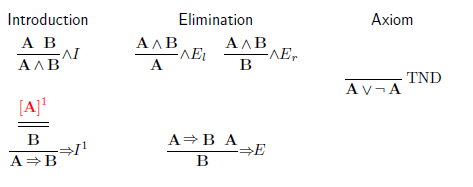
\includegraphics[scale=0.8]{figures/295}
\end{figure}
\begin{figure}[H]
            \centering
            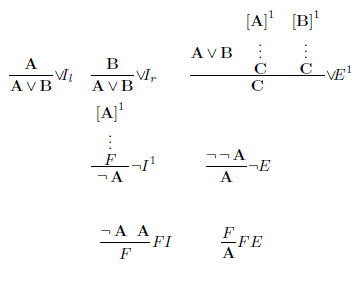
\includegraphics[scale=0.8]{figures/298}
\end{figure} 
\subsubsection{Analytical Tableaux}
\begin{itemize}
    \item
        $A^{\alpha}$, with $\alpha \in \{T, F\}$ is called a labeled formula
    \item
        $\Phi$ set of formulae, $\Phi^{\alpha} = \{A^{\alpha} | A \in \Phi\}$
    \item
        Idea: instead of $\emptyset \vdash Th$, show $\lnot Th \vdash \bot$
    \item
        Analyzed in a tree to determine satisfiability
    \item
        Branches correspond to valuations (models)
        \begin{figure}[H]
            \centering
            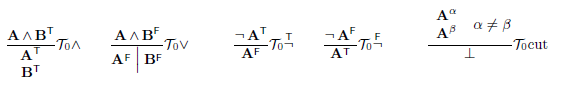
\includegraphics[scale=0.8]{figures/302}
        \end{figure}
    \item
        Saturated tableau: no rule yields anymore new results
    \item
        Closed branch: ends on $\bot$ (closed tableau: every branch is closed)
    \item
        Open branch yields model in saturated tableaux
    \item
        $A$ is a $T_0$ theorem ($\vdash_{T_0} A$), iff there is a closed tableaux with $A^F$ at root
    \item
        $\Phi \subseteq wff_0(V_0)$ derives $A$ in $T_0$ ($\Phi \vdash_{T_0} A$), iff there is a closed tableau starting with $A^F$ and $\Phi^T$
\begin{figure}[H]
            \centering
            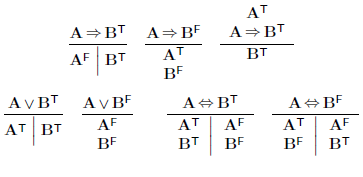
\includegraphics[scale=0.8]{figures/308}
\end{figure} 
\end{itemize}
\subsubsection{Resolution}
\begin{itemize}
    \item
        Operates on single inference rule:
\begin{figure}[H]
            \centering
            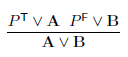
\includegraphics[scale=0.8]{figures/312}
\end{figure} 
    \item
        Let $S$ be a clause set, then we call a $R$ derivation $D: S \vdash_R \square$ a resolution refutation
    \item
        Resolution proof: We call a resolution refutation of $CNF(A^F)$ a resolution proof
\end{itemize}
\end{document}

